\section{Metodologia e metas}
\subsection{A Estrutura Analítica do Projeto - EAP}

A EAP é uma representação sistêmica do projeto que evidencia seus principais 
resultados, bem como as fases necessárias a sua conclusão. As imagens 
apresentadas a seguir representam a visão geral da EAP do projeto.

\newpage
%-------------------------------------------------------------------------------
\begin{landscape}
\begin{figure}[]
\centering
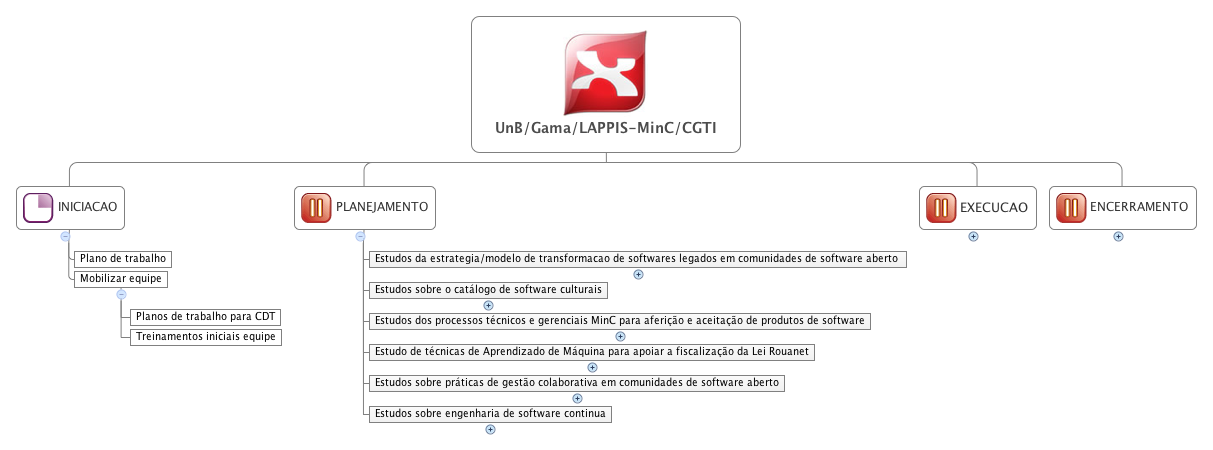
\includegraphics[keepaspectratio=true,scale=0.55]{figuras/UnB-Gama-LAPPIS-MinC-CGTI-Ini-Plan.png}
\caption{Visão dos resultados fase de iniciação e planejamento}
\label{figura-eap_iniciação}
\end{figure}
\end{landscape}

\begin{landscape}
\begin{figure}[]
\centering
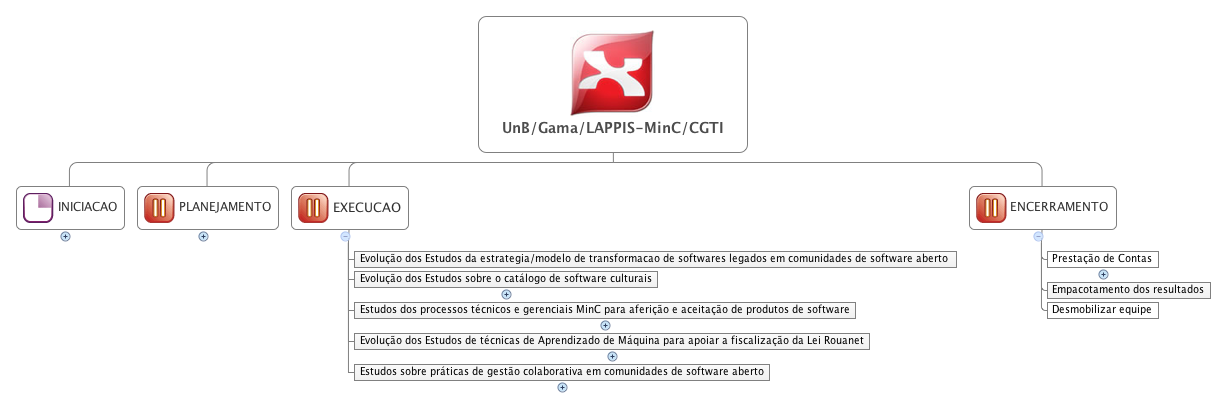
\includegraphics[keepaspectratio=true,scale=0.55]{figuras/UnB-Gama-LAPPIS-MinC-CGTI-Exec-Enc.png}
\caption{Visão dos resultados fase de execução e encerramento}
\label{figura-eap_planejamento}
\end{figure}
\end{landscape}


Elencamos os principais resultados observárveis que serão gerados no decorrer 
deste projeto e alinhadas com o objeto e metas propostas no projeto.


\subsubsection{Pacote de Trabalho: Estratégia/modelo de transformação de 
softwares legados em comunidades de software aberto}

Evoluir e manter um software legado é uma experiência desgastante para 
desenvolvedores e desestimulantes no contexto de fomento a comunidades. Por outro lado, 
a reescrita desses softwares é impraticável e, em se tratando de software implantado,
a necessidade de adicionar novas funcionalidades e dar manutenção persiste. 

Muito sistemas legados carecem testes automatizados, boa documentação e práticas 
de desenvolvimento contínuo, o que dificulta enormemente qualquer forma de evolução.
Estes também são fatores críticos na curva de aprendizado de novos desenvolvedores
e criam uma barreira para a existência de comunidades de software livre/aberto 
colaborando com tais sistemas.  

As práticas modernas de manutenção e evolução de software tornaram difusas várias linhas 
entre o desenvolvimento e a operação do sistema. Neste contexto, foi cunhado o termo DevOps para 
os profissionais que trabalham nesta zona de interface utilizando técnicas de desenvolvimento
de software para automatizar os processos de implantação e execução do sistema 
\cite{deFranca:2016:CDH:2973839.2973845}. O objetivo dessa etapa é utilizar os
conceitos e práticas Devops no contexto de software legado.

Será realizada uma pesquisa exploratória tendo como objeto de estudos estudos 
das práticas atuais de desenvolvimento e implantação de sistemas legados no 
Ministério da Cultura, visando promover o alinhamento com práticas modernas de 
automação e DevOps aplicadas, na medida do possível, em sistemas legados. 
Este ciclo de desenvolvimento possui um papel estratégico duplo. Por um lado, 
integra-se ao ciclo de formação dos alunos de Engenharia de Software capacitando 
alunos em metodologias e tecnologias favorecidas pelo LAPPIS em casos de uso reais. 
Estas tecnologias são estratégicas na filosofia de desenvolvimento aplicada no 
laboratório e envolvem temas como conteinerização, receitas, versionamento, gerência
de repositórios, testes automatizados, entre outros. Além disso, a implementação
de um fluxo de trabalho DevOps é um requisito para que seja possível apropriar, 
integrar e evoluir sistemas legados de forma isolada e com com riscos mínimos. 

Alguns sistemas legados mantidos pelo MinC serão usados como estudo de casos, tais 
como SIMEC, Salic e Sistel. A escolha dos sistemas a serem usados no estudos de 
caso será feita em conjunto com a equipe do Ministério da Cultura, de acordo com 
os interesses e necessidades mútuas.

Esta etapa implicará na criação de um relatório com os principais resultados 
encontrados, assim como sugestões de boas práticas para a correção destes problemas. 
 
Tal resultado será de grande relevância, tanto para a equipe  de TI do Ministério 
da cultura quanto comunidade acadêmica, uma vez que guia desenvolvedores e gestores 
a organizarem o processo de refatoração de sistemas legados, a fim de minimizar 
os esforços requeridos e maximizar os resultados efetivos \cite{Khanam2017refact}.

São objetivos para a Etapa:

\begin{itemize}
 \item Estudos e documentação do processo de conteinerização, testes automatizados, 
  refatoração de sistemas legados em uma estrutura de DevOps para viabilizar trabalhos futuros;
\item Pesquisa em metodologias de refatoração de sistemas legados;
\item Utilizar como estudo de casos alguns sistemas legados do Ministério da 
  Cultura, tais como o projeto SIMEC (Sistema Integrado de Monitoramento Execução 
  e Controle) e o projeto Salic (Sistema de Apoio às Leis de Incentivo à Cultura), Sistel. 
\end{itemize}


\subsubsection{Pacote de Trabalho: Estudo sobre catálogos de Software Culturais}

Nessa etapa será realizado o desenvolvimento do Catálogo de Software do Ministério 
da Cultura. Hoje, o Ministério da Cultura conta somente com uma conta pública 
github\footnote{\url{https://github.com/culturagovbr}}, para disponibilzar os 
softwares abertos desenvolvidos e mantidos pela equipe de TI. Tais projetos não 
possuem padronização de documentação e, algumas vezes, não possuem sequer licença de software. 

O foco dessa etapa é executar o ciclo de projeto de software completo, desde a iniciação.
Assim, o projeto já será iniciado como software livre e com as práticas de devops, 
ferramentas e tecnologias modernas. Será focado o levantamento das tecnologias e 
ferramentas usadas pela comunidade de software livre para automatizar o processo de 
desenvolvimento e implantação do software, pois há pouca pesquisa focada nesse 
tema \cite{DBLP:conf/icse/KrafftSF16}. O principal objetivo nessa etapa é exercitar 
em todo ciclo de projeto a experimentação e inovação contínua \cite{DBLP:journals/jss/FitzgeraldS17, DBLP:conf/icse/KrafftSF16}, 
de forma a subsidiar a pesquisa realizada na Etapa 5 (Sec. \ref{Sub:etapagerenciais}). Um objetivo
secundário dessa fase é o mapeamento do portfólio de software mantido pela equipe 
do MinC e o levantamento de requisitos para que esses repositórios (licenças, 
documentação, organização, estruturação) sigam padrões aceitáveis nas comunidades 
de software livre. Espera-se que o resultado dessa pesquisa possa colaborar tanto 
com a comunidade acadêmica quanto a de desenvolvedores de software livre. 

São objetivos para a Etapa:

\begin{itemize}
  \item Aplicação de práticas de experimentação e inovação contínua no 
    desenvolvimento do projeto de Catálogo de Software Culturais;
  \item Realizar estudos e documentação do processo de desenvolvimento e das boas 
    práticas e automações realizadas;
  \item Relatório com os  modelos de desenvolvimento e comunidade para serem 
    aplicados aos projetos de software do Minc
  \item Transferência de conhecimento e capacitar a equipe de servidores e técnicos 
  do MinC em práticas de gestão e desenvolvimento de software aberto, colaborativo e contínuo.
\end{itemize}

\subsubsection{Pacote de Trabalho: Estudos sobre práticas de gestão colaborativa 
em comunidades de software aberto}

Nessa etapa será realizada uma pesquisa exploratória tendo como objeto de estudo 
os movimentos, organizações, desenvolvedores e demais stakeholders que atuam na gestão
colaborativa de software aberto. O principal objetivo do trabalho de gestão colaborativa
dessas comunidades de software aberto é manter um conjunto de ações de governança 
digital e comunicação que aproveite ao máximo esse potencial em favor das necessidades
do órgão e das metas comuns às organizações parte das comunidades. Esse esforço 
envolve um trabalho de mapeamento de atores de cada comunidade (atuais e 
potenciais futuros), assessoria para planejamento conjunto, facilitação de fluxos 
de comunicação e mobilização, realização de atividades conjuntas para integração, 
identificação de oportunidades externas, assessoria para comunicação e divulgação 
ao público externo à comunidade e apoio para solução de conflitos.

Além desses estudos e práticas, as ações de governança digital empreendidas nas 
comunidades do catálogo de softwares de gestão cultural do MinC irão subsidiar 
outras partes do projeto, principalmente os esforços ligados à engenharia de software 
contínua, como contribuindo na definição da participação dos atores da comunidade nos
processos de planejamento e monitoramento contínuo.

O principal resultado dessa pesquisa será sistematizar e produzir conhecimento 
sobre as práticas das comunidades de software livre que o Estado participa por 
adesão e, a partir dos aprendizados com seus arranjos, orientar e capacitar 
os servidores e técnicos do MinC nas práticas de 
planejamento, gestão de softwares abertos, aprimorando os mecanismos de 
governança digital dos softwares presentes no portifólio do MinC.

São objetivos para a Etapa:

\begin{itemize}
  \item Estudos de caso sobre comunidades de software livre onde o Estado 
    participa por adesão, com prioridade para os softwares utilizados para a gestão cultural;
  \item Estudos sobre boas práticas para planejamento conjunto de milestones e 
    releases entre as organizações que fazem parte das comunidades;
  \item Estudos sobre boas práticas de comunicação e mobilização no contexto das 
    comunidades onde o Estado participa;
  \item Participação em eventos e encontros das comunidades de software livre 
    que contribuem para o portifólio mantido pelo MinC;
  \item Estudos sobre arranjos econômicos utilizados pelas comunidades com fins 
    de sustentabilidade de seus comuns de software;
  \item Estudos sobre metodologias e suportes tecnológicos para a gestão colaborativa 
    em comunidades de software livre nas quais o Estado participa por adesão.
\end{itemize}


\subsubsection{Pacote de Trabalho: Estudo de técnicas de Aprendizado de Máquina 
para apoiar a fiscalização da Lei Rouanet}

O aumento exponencial na capacidade de processamento e armazenamento nos 
últimos anos viabilizou várias técnicas de processamento de dados que extrapolam
os relatórios simples de caráter descritivo e tentam incorporar inteligência
de máquina na análise e nos processos decisórios. O conjunto destas técnicas é
conhecido de forma difusa como "aprendizado de máquina" e incorpora tanto métodos
estatísticos, como de processamento de linguagem natural, compressão de dados, redes 
neurais, etc. Estes métodos estão cada vez mais populares na indústria e fomentam
vários mecanismos de automação e inteligência de negócios.

De  1992-2017, 16 bilhões de reais foram captados via a Lei Federal 8.313/91 de 
Incentivo à Cultura, mais conhecida como lei Rouanet. Para ser beneficiado com 
captação de recurso via lei Rouanet, o proponente passa por duas etapas: a  etapa 
de habilitação e a etapa  de prestação de contas. Ambas etapas são realizadas 
com o uso da plataforma SALIC (Sistema de Apoio às Leis de Incentivo à Cultura)
\footnote{\url{http://salic.cultura.gov.br/autenticacao/index/index}}. 

Atualmente, a conformidade das submissões com a lei é realizada manualmente por 
avaliadores/auditores. A grande quantidade de propostas torna muito difícil 
a análise minuciosa para detecção de fraudes no processo, tanto na etapa de 
habilitação quanto na etapa de prestação de contas. O uso de técnicas de 
aprendizado de máquina pode auxiliar tanto o proponente nas dúvidas encontradas 
no processo de submissão de proposta, quanto o auditor, na detecção de possíveis 
anomalias dos projetos submetidos na plataforma.

O principal objetivo é o estudo de técnicas de Aprendizado de Máquina que possam 
apoiar o sistema de recomendação e fiscalização da lei Rouanet. Nessa etapa será realizada 
uma pesquisa exploratória em técnicas de aprendizado de máquina e processamento 
de linguagem natural. Tais técnicas e algoritmos serão aplicados para melhorar a 
experiência de usuário (UX) por meio da proposta de chatbots como interface entre 
os proponentes na lei Rouanet e o Ministério da Cultura. 

Além disso, técnicas de aprendizado de máquinas serão estudadas para automatizar 
processos nas trilhas de auditorias, tanto na etapa de habilitação e aprovação, 
quanto na etapa de prestação de contas. O objetivo é auxiliar auditores a 
encontrar erros, inconsistências e detecção de anomalias nas submissões. 

Por fim, a massa de dados correspondente ao histórico de proposições, pode ser 
analizados, minerados, extraído padrões, a fim de inferir informações
a partir dos dados, de forma a auxiliar na tomada de decisão estratégica.

Essa pesquisa exploratória, usaremos bibliotecas de aprendizado de máquina e 
processamento de linguagem natural em código aberto, tais como scikit-learn 
\footnote{\url{https://github.com/scikit-learn/scikit-learn}} e Tensorflow 
\footnote{\url{https://github.com/tensorflow/tensorflow}}, NTLTK
\footnote{\url{https://nltk.org/}}, que atualmente são 
utilizadas tanto pela comunidade acadêmica quanto pela indústria de software.  

São objetivos para a Etapa:

\begin{itemize}
 \item Realizar estudos e propor técnicas de processamento de linguagem natural, 
  aprendizado supervisionado e o desenvolvimento de chatbots para interagir
  com proponentes da Lei Rouanet;
 \item Realizar estudos e propor técnicas de aprendizado supervisionado e 
  detecção de anomalias para automatizar as trilhas de auditoria na fase de 
  aprovação e prestação de contas;
 \item Realizar estudos e propor técnicas de reconhecimento de padrão e 
  Inteligência de Negócio para análise dos projetos submetidos via Lei Rouanet;
\end{itemize}


\subsubsection{Pacote de Trabalho: Visualização de dados e criação de Dashboards}

O processamento de grandes volumes de dados pressupõe a necessidade de identificar
padrões e informações úteis. Muitas vezes a forma mais conveniente de apresentar
estes dados é na forma de gráficos ou outros recursos visuais.

O tema deste estudo é buscar formas visuais de apresentar os dados obtidos e 
processados nas etapas anteriores. Os gráficos produzidos servem de embasamento
tanto para análise por parte da equipe do projeto quanto pelos gestores do próprio
ministério.

São objetivos para a Etapa:

\begin{itemize}
 \item Painéis com estatísticas sobre projetos cadastrados no Salic.
 \item Estudos sobre a apresentação visual de resultados de algoritmos de aprendizado
  de máquina e análises estatísticas. 
 \item Dashboard  para a visualização e análise das relações entre proponentes 
  e financiadores por meio de grafos.
\end{itemize}


\subsubsection{Pacote de Trabalho: Estudos dos processos técnicos e gerenciais 
MinC para aferição e aceitação de produtos de software}
\label{Sub:etapagerenciais}

O objetivo geral desta frente de pesquisa é auxiliar os times de desenvolvimento 
e gestores de TI do MinC a aprimorarem sua capacidade em tomar decisões acerca 
da qualidade das versões dos produtos de software entregues por seus fornecedores. 

São objetivos para a Etapa:

\begin{itemize}
 \item  Experimentação contínua aplicada à engenharia de produto de software;
 \item a mineração em repositórios de software e a análise científica de dados do software
 \item prospectar uma sistemática, baseada em evidência científica, que auxilie 
  a homologação de produtos de software, em obediência ao normativo estabelecido.
\end{itemize}
